% ****** Start of file apssamp.tex ******
%
%   This file is part of the APS files in the REVTeX 4.1 distribution.
%   Version 4.1r of REVTeX, August 2010
%
%   Copyright (c) 2009, 2010 The American Physical Society.
%
%   See the REVTeX 4 README file for restrictions and more information.
%
% TeX'ing this file requires that you have AMS-LaTeX 2.0 installed
% as well as the rest of the prerequisites for REVTeX 4.1
%
% See the REVTeX 4 README file
% It also requires running BibTeX. The commands are as follows:
%
%  1)  latex apssamp.tex
%  2)  bibtex apssamp
%  3)  latex apssamp.tex
%  4)  latex apssamp.tex
%
\documentclass[%
 reprint,
%superscriptaddress,
%groupedaddress,
%unsortedaddress,
%runinaddress,
%frontmatterverbose, 
%preprint,
%showpacs,preprintnumbers,
%nofootinbib,
%nobibnotes,
%bibnotes,
 amsmath,amssymb,
 aps,
%pra,
%prb,
%rmp,
%prstab,
%prstper,
%floatfix,
]{revtex4-1}

\usepackage{multirow}
\usepackage{verbatim}
\usepackage{graphicx}% Include figure files
\usepackage{dcolumn}% Align table columns on decimal point
\usepackage{bm}% bold math
\usepackage{hyperref}% add hypertext capabilities
\usepackage{listings}% code listings
%\usepackage[mathlines]{lineno}% Enable numbering of text and display math
%\linenumbers\relax % Commence numbering lines

%\usepackage[showframe,%Uncomment any one of the following lines to test 
%%scale=0.7, marginratio={1:1, 2:3}, ignoreall,% default settings
%%text={7in,10in},centering,
%%margin=1.5in,
%%total={6.5in,8.75in}, top=1.2in, left=0.9in, includefoot,
%%height=10in,a5paper,hmargin={3cm,0.8in},
%]{geometry}

\lstdefinestyle{custompython}{
  belowcaptionskip=1\baselineskip,
  breaklines=true,
  frame=L,
  xleftmargin=\parindent,
  language=Python,
  showstringspaces=false,
  basicstyle=\footnotesize\ttfamily,
}

\begin{document}

\preprint{APS/123-QED}

\title{Modeling Information Diffusion in Faculty Hiring Networks}% 
\thanks{Aaron Clauset, Sam Way}%

\author{Dimitrios Economou}%
 \email{Dimitrios.Economou@colorado.edu}
\author{Allison Morgan}%
 \email{Allison.Morgan@colorado.edu}
\affiliation{%
 Department of Computer Science, University of Colorado, Boulder, CO 80303, USA
}%

\collaboration{Network Analysis \& Modeling Final Project}%\noaffiliation

\date{\today}

\begin{abstract}
Faculty hiring networks exhibit strong institutional hierarchies with high prestige universities populating faculty positions at all prestige levels. In this paper, we study the effect of this core-periphery structure on the influential power of institutions under various epidemic models. We find that institutional prestige has a significant impact on the spread of ideas in these networks. Ideas originating from lower prestige institutions have to be higher in quality in order to achieve similar success as lesser quality ideas originating from higher prestige institutions.
\end{abstract}

\maketitle

\section{\label{sec:level1}Introduction}

Previous sociology of science work has suggested that researchers from high ranking institutions have large influence over scientific communication. Hagstrom found significant correlation between department prestige and research production and citation levels. He also notes prestigious departments' roles as central players: ``Scientists in high prestige departments tend to be centrally located with regard to scientific communication; not only do they publish more, but they engage more frequently in the informal circulation of manuscripts''~\cite{hagstrom:prestige}. Similarly, Cole has suggested that the contributions of these prestigious departments are more visible. Though prestige appears to have no impact for high quality papers, ``lesser quality papers by high-ranking scientists receive greater attention than papers of equal quality by low-ranking scientists''~\cite{cole:citation-prestige}. Cole's work examines the ``Matthew Effect,'' in which well-known scientists receive more credit than lesser-known scientists for comparable (in quality) contributions~\cite{merton:matthew-effect}. Furthermore, the prestige of a researcher's department has been shown to have a substantial effect on their productivity rate and citation count. Allison and Long showed that faculty members who take positions at departments of higher prestige, see a substantial increase in their productivity and citation levels, whereas a significant decrease in those levels was observed for those who take a position at a department of lower prestige~\cite{allison:department-effects}. This finding suggests that faculty hiring and placement have a profound effect on the amount of research produced and its visibility. In this paper, we simulate information diffusion on faculty hiring networks, which as Allison and Long suggests, act as a conduit for the spread of ideas~\cite{allison:department-effects}.

\subsection{\label{sec:level2}Faculty Hiring Network}

Our analysis relies on a hand-collected data set of faculty career trajectories from 462 computer science, business, and history departments from North American universities~\cite{clauset:hiring, clauset:hiringweb}. This data was used to build three multi-edge, directed faculty hiring networks. A node in these networks is a university. There exists an edge $(u, v)$ if a faculty member received their Ph.D. from university $u$ and subsequently took a tenure-track position at university $v$. Universities may have many edges between them, representing the multiple faculty candidates produced by a university $u$ who later landed a position at university $v$. These networks also contains self-loops, which correspond to people who received their Ph.D. at a particular institution and took a faculty job at the same institution. We have omitted the node (and edges into or out of that node) representing all non-Ph.D. granting universities from our analysis.

\subsection{\label{sec:level2}Prestige}
For any directed graph $G = (V, E)$, we define a \emph{prestige hierarchy} $\pi : V \to [1, \infty)$, where $\pi_u = 1$ is the rank of the highest prestige vertex $u$. A hierarchy $\pi$'s \emph{strength} $\rho$ is defined to be the fraction of edges $(u, v)$ in $E$ such that $\pi_u \leq \pi_v$, maximized over all possible rankings on $V$. To extract consensus prestige hierarchies for each of the three faculty hiring networks, Clauset et al. sampled optimal rankings and took averages for each node rank in each sampled ranking of maximal $\rho$. This resulted in significantly strong prestige hierarchies, in which ``only 9 to 14\% of faculty are placed at institutions more prestigious than their doctorate ($\rho = 0.86$ to $0.91$),'' noting that $\rho = 1$ represents a perfect hierarchy. Further, they showed that these rankings were as accurate in estimating institutional prestige as authoritative rankings such as U.S. News \& World Report and National Research Council rankings~\cite{clauset:hiring}. These prestige rankings are publicly available in the same data set and are what we used in this study.

\subsection{\label{sec:level2}Core-periphery Structure}

In previous work, it was suggested that in each of these three faculty hiring networks, there exists a strong core-periphery structure where the most prestigious universities occupy central positions within the network~\cite{clauset:hiring}. To lend further support for this conclusion, we have shown in Fig.~\ref{centrality} that across all departments, closeness centrality is the largest for high prestige universities and steadily decreases with decreasing university prestige. (Universities with closeness centralities of 0 have no outward edges from them. These universities may have either produced no tenure-track faculty members, or their faculty were placed at non-Ph.D. granting institutions.)

Another way of visualizing this structure is to look at the density of edges between universities. In Fig.~\ref{adjacency}, we have shown the counts of edges between Ph.D. granting and faculty placement institutions. Universities are binned by prestige such that the top 10\% reside in the upper leftmost corner of each matrix. Across all three departments, we can see that most faculty members have received their Ph.D.'s from the top universities (indicated by their dark top rows). Furthermore, there is a strong upper triangular trend: faculty rarely take positions at institutions of higher rank than their Ph.D. granting institutions. In other words, those who take positions at high prestige universities very rarely received their Ph.D. from an institution of lower prestige. These results are consistent with the findings from Clauset et al.~\cite{clauset:hiring}.

\begin{figure}[h]
\centering
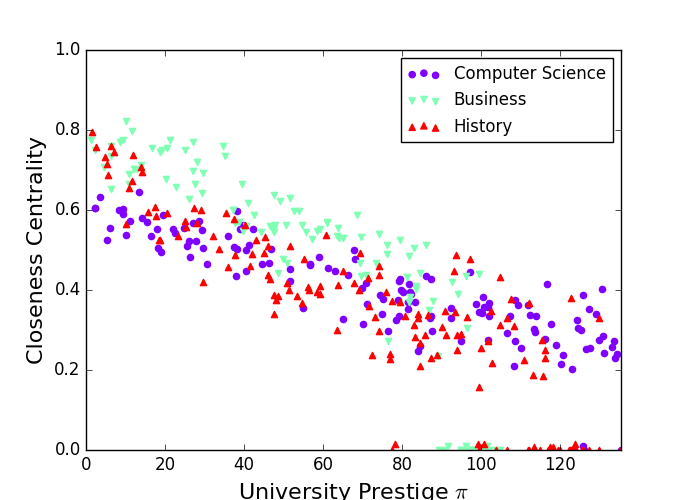
\includegraphics[width=0.5\textwidth]{figures/centrality.png}
\caption{Closeness centrality for every university in the computer science, business, and history faculty hiring networks. Each university has an associated prestige, plotted above.}
\label{centrality}
\end{figure}

\begin{figure*}
	\centering
  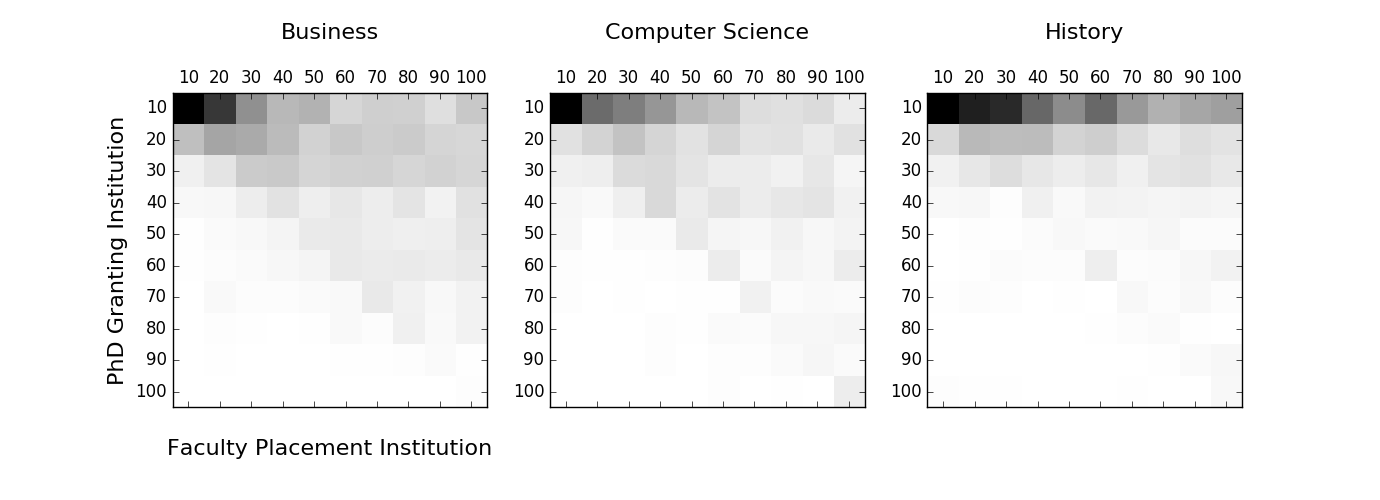
\includegraphics[width=\textwidth]{figures/grouped_adjacency.png}
  \caption{Adjacency matrices for each department. Universities of similar prestige are grouped together, such that rows (Ph.D. granting institutions) and columns (faculty placement institutions) reflect the top 10\%, 20\%, etc. Shading reflects the density of edges between two groups of universities.}
   \label{adjacency}
\end{figure*}

\section{\label{sec:level1}Methods}
\subsection{\label{sec:level2}Software Used}
We use NetworkX~\cite{networkx} to construct our networks and simulate epidemics on them, NumPy~\cite{numpy} for basic numerical analysis, and SciPy~\cite{scipy} for curve fitting.

\subsection{\label{sec:level2}Epidemic Models}

We restricted our analysis to three epidemic models: SI, SIR, and SIS~\cite{newman:networks}. The spread of ideas via all three models represent the spread of research ideas across faculty hires. Initially, we infect a single university and then run one of the epidemic models, recording the resulting epidemic's \emph{size} (the fraction of infected nodes) and \emph{length} (the number of time steps) when the infection has stopped spreading. Since each university has a prestige ranking, we can assess the success of the idea in spreading throughout the network as a function of the initial university's prestige.

The simplest epidemic model SI consists of just two node-level states: susceptible and infected. SI allows for no remission from infections. In other words, once a university gains at least one faculty member working on a research idea, that university remains infected over the lifetime of the epidemic (the idea continues to be worked on by other members). Other epidemic models considered allow for recovery (SIR) and repeated returns to susceptible states (SIS).

The SIR model permits nodes to recover from an infection (via immunity or removal from the population). In the faculty hiring networks, a university may ``recover'' from an idea when faculty working within a particular research area retire, lose interest, or lose funding. The SIS model allows nodes to become susceptible to re-infection. This scenario might represent faculty taking a brief break from their research (e.g. parental leave). What follows next is a brief summary of the inner working of our models.

Initially, we infect a single university. At each time-step, for each infected university $u$, each of $u$'s susceptible neighbors has a chance of $p$ to contract $u$'s infection. Each edge in the network gets at most one chance at spreading the infection. The constant probability $p$ at which an infection (idea) spreads is referred to as the \emph{infection probability}, and we interpret it as the \emph{fitness} or quality of the idea. Higher quality or fitter ideas will be more likely to spread across faculty hires.

In the SIR and SIS models, at each time-step, each infected node has a fixed chance of $r$ to recover (in the case of SIR) or become susceptible again (in the case of SIS). We call the likelihood $r$ of recovering from an infection the \emph{recovery probability}. In our analysis, we consider the \emph{spreading parameter} $p/r$ (also called the \emph{basic reproduction number}) to represent the fitness of ideas \cite{jones:reproduction}. For example, a spreading parameter of $5$ means that idea proliferation is $5$ times as likely as idea recovery, while a spreading parameter of $1/2$ means that idea recovery is twice as likely as idea transmission. This makes sense if we interpret recovery as faculty members no longer working on a particular idea.

We chose to only demonstrate the ratio $p/r$ and not also more exhaustive combinations of $p$ and $r$. We did so initially for robustness, but found that the results did not convey any additional useful information. This is in line with results from Chakrabarti et al.~\cite{chakrabarti:epidemicsonrealnetworks} that say that $p/r$ is all that matters for the SIS model. They suspect the same is true for SIR, but more investigation is required for certainty. An inspection of the literature shows that people studying the SIR model on networks also consider the ratio $p/r$~\cite{fournet:2016,jones:reproduction}. \\

\subsection{\label{sec:logistic}Logistic Model}

For any given infection probability $p$, we model the effect of the initially infected university's prestige $\pi$ on the resulting epidemic's size $s : [1, \infty) \to [0, 1]$ as
\[
  s(\pi) = \frac{s_\text{max}}{1 + e^{-k (\pi - \pi_\text{mid})}},
\]
where $s_\text{max}$ is the upper bound of the size, $k$ is the growth rate, and $\pi_\text{mid}$ is the symmetric inflection point. Note that smaller $\pi$ corresponds to higher prestige (with $1$ being the highest prestige), so we get negative growth rates $k$. We used SciPy's non-linear least squares fitting function \texttt{optimize.curve\_fit} for the fitting \cite{scipy}.

%\textbf{TODO}: \href{https://en.wikipedia.org/wiki/Generalised_logistic_function}{glf}  ... If we have time, it might be interesting to play around with more general logistic curves for better fits. Otherwise, we can just mention that we can look into this in the future.

\section{\label{sec:level1}Results}
\subsection{\label{sec:level2}Susceptible-Infected}

%\textbf{TODO: report curve parameters and discuss.. $\pi_{mid}$ and $k$ especially and make remarks on them}\\ 

In Fig.~\ref{SI-size}, we have plotted epidemic size versus prestige for various infection probabilities. Across disciplines, higher prestige universities infect more of the population at lower infection probabilities (idea fitness) as compared to low prestige universities. In our real-world analogy, this conveys that low quality research ideas generated at high rank institutions gain more traction than similar quality ideas generated at lower ranked institutions, consistent with Cole's earlier mentioned work \cite{cole:citation-prestige}. We can also see that increasing the fitness of an idea has more of an effect on epidemic size if the idea starts at lower prestige institutions. We will investigate this phenomenon more in section~\ref{sec:infection}.

We fit logistic curves (described in section~\ref{sec:logistic}) to model the effect of the prestige of the first infected university on epidemic size. The reasonably good fit of this model to these results shows that for any given idea fitness, there is a certain prestige $\pi_\text{mid}$ at which there is an exponential change in epidemic size in response to a change in prestige around $\pi_\text{mid}$. We can see that increasing the fitness of the idea shifts the inflection point $\pi_\text{mid}$ to a lower prestige and increases the exponential rate of change in size around that point. This simply means that ideas at those lower prestige institutions (near $\pi_\text{mid}$) are now suddenly finding much greater success than they were with less fit ideas. We will later see that this same fact holds for the SIR and SIS models and we therefore will not comment on it in those upcoming sections.

Consistent with this finding, we observe that infections starting from low ranked universities tend to die out quicker than those initiated from high ranked universities as shown in Fig.~\ref{SI-length}. Here, we plot a \emph{normalized epidemic length}: the epidemic length divided by the average shortest path length from a node, which we interpret as how far an idea is likely to go given the network structure. This measure tells us how long an idea circulates given how much that circulation is constrained. We generally see that ideas are in circulation longer if they originate from higher prestige institutions. However, as the infection probability increases, the epidemic length approaches a value constant across prestige. This finding suggests that at some high enough infection probability (roughly 0.9), every university spreads its ideas as much as it possibly can.

\begin{figure*}
	\centering
  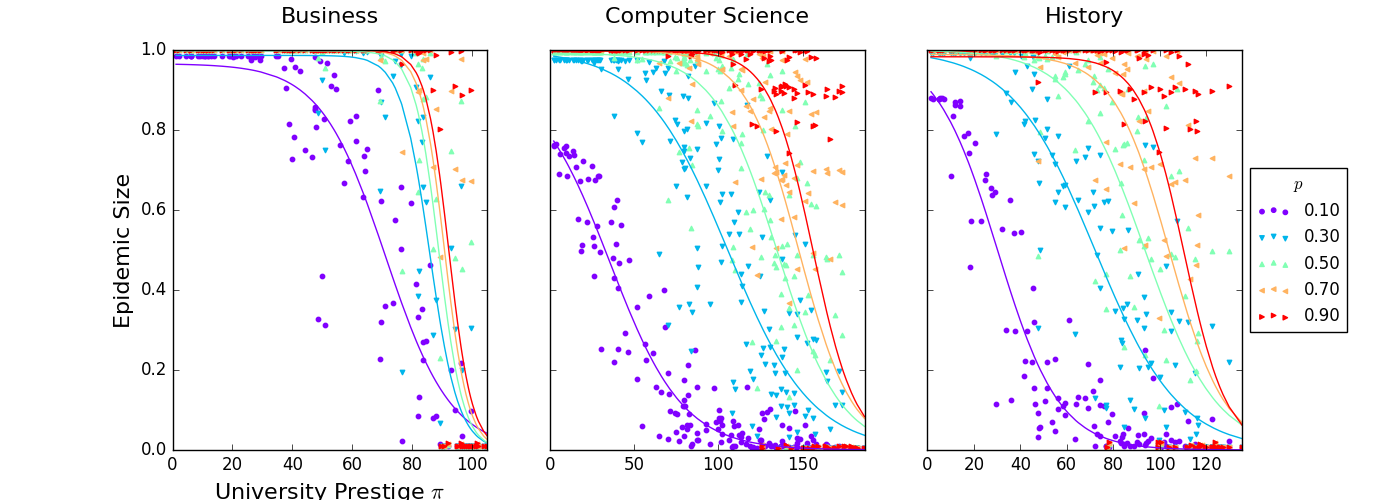
\includegraphics[width=\textwidth]{figures/size-results-of-ALL-SI.png}
  \caption{Epidemic size versus prestige of the initially infected node under the SI model for all three departments. Each data point represents an average result over 1000 trials of the simulation. Colors correspond to different infection probabilities.}
  \label{SI-size}
\end{figure*}

\begin{figure*}
	\centering
  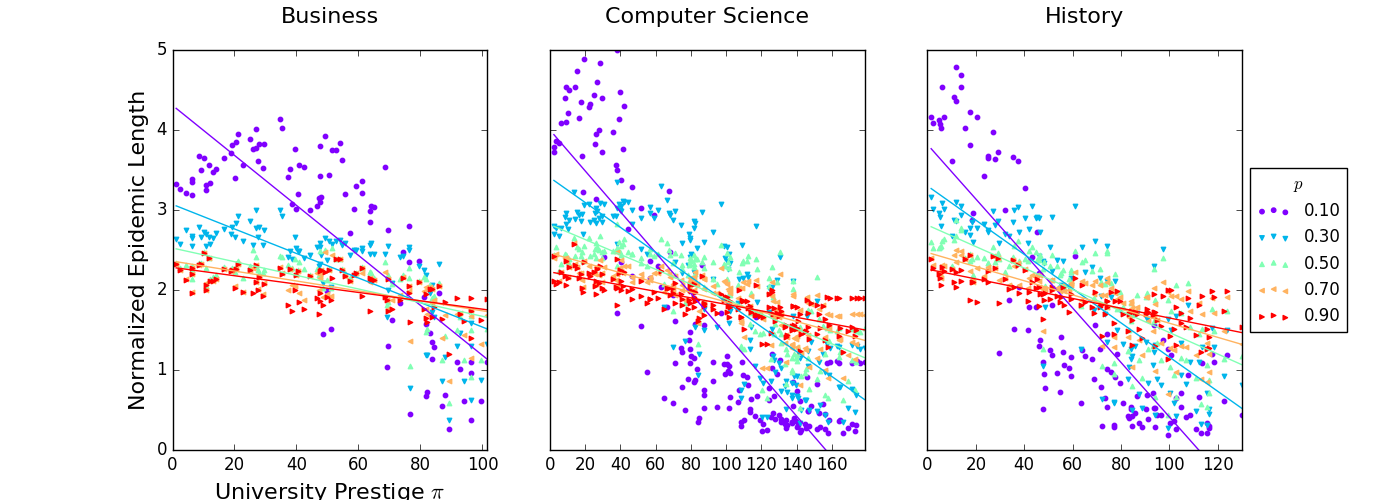
\includegraphics[width=\textwidth]{figures/length-results-of-ALL-SI.png}
  \caption{Normalized epidemic length versus prestige of the initially infected node under the SI model for all three departments. Each data point represents an average result over 1000 trials. Again, colors correspond to different infection probabilities.}
   \label{SI-length}
\end{figure*}

\subsection{\label{sec:level2}Susceptible-Infected-Recovered}

In the second epidemic model considered, we observe similar trends to what we saw with SI. The difference, as seen in Fig.~\ref{SIR-size}, is that epidemic size is generally smaller than it was under SI for all departments. This result is to be expected since at every time-step, each infected node has a chance to recover. Thus, at the end of an epidemic, many nodes may have recovered and less nodes will remain infected. Another interesting thing to note about this figure is that for the business discipline, the ``plateau'' is longer and remains more flat across fitness of ideas than the other disciplines. This is consistent with some of Clauset et al.'s findings that the business discipline's hiring network was slightly more ``equal'' and less hierarchical than the others.

Generally, normalized epidemic length is also shorter under SIR model than it was under SI, as shown in Fig.~\ref{SIR-length}. By allowing nodes to recover with immunity, we restrict the number of nodes which can transmit the infection. Thus, the infection is likely to die out quicker under this model. One interesting feature of Fig.~\ref{SIR-length} that we do not see in Fig.~\ref{SI-length} and Fig.~\ref{SIS-length} is that the fitness $p/r$ of the idea does not have much of an effect on the higher prestige institutions than it does on the lower prestige institutions. This means that regardless of the quality of the idea, it will remain in circulation for longer than lower prestige institutions. However, if the idea starts at a lower prestige institution, then the fitness of the idea has real impact on how long the idea circulates in the networks. 

However, under this model, we still see similar effects of prestige on epidemic size as we saw with the SI model: the less prestigious the university an idea starts at is, the less amount of universities the idea spreads to, and the quicker the idea dies off. Further, increasing the fitness of the idea has more of an effect if the idea starts at lower prestige institutions.

\begin{figure*}
	\centering
  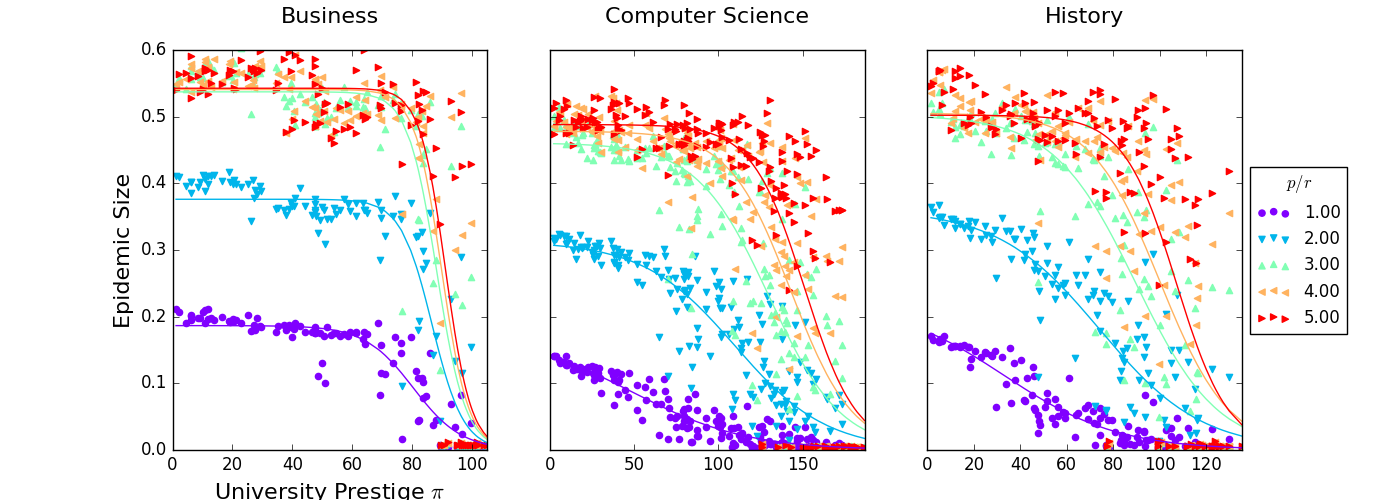
\includegraphics[width=\textwidth]{figures/size-results-of-ALL-SIR.png}
  \caption{Epidemic size versus prestige of the initially infected node under the SIR model, averaged over 500 trials.}
    \label{SIR-size}
\end{figure*}

\begin{figure*}
	\centering
  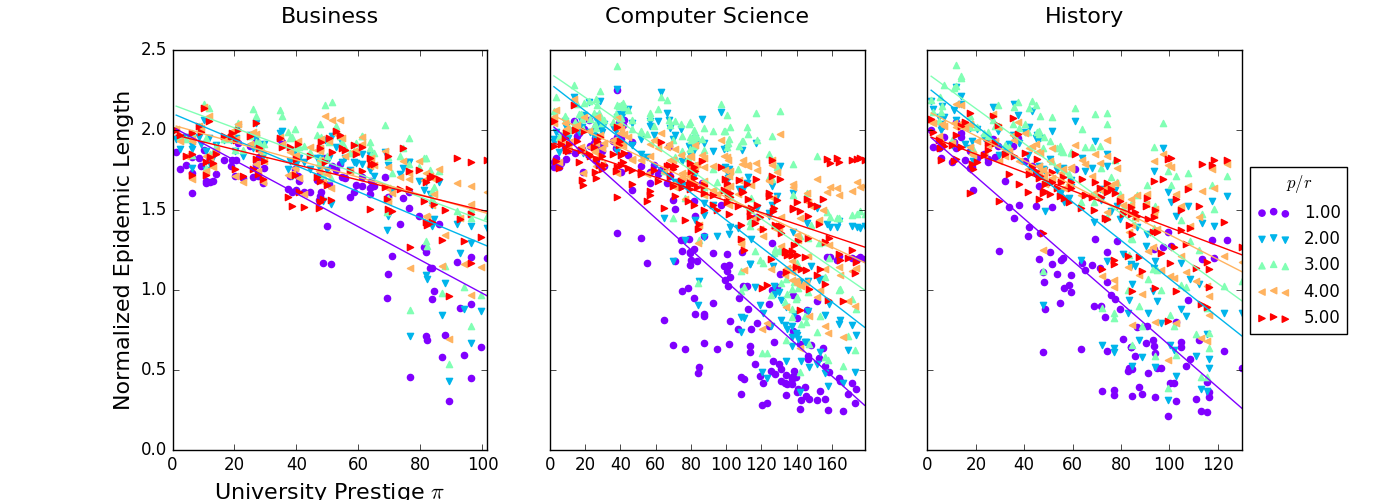
\includegraphics[width=\textwidth]{figures/length-results-of-ALL-SIR.png}
  \caption{Normalized epidemic length versus prestige of the initially infected node under the SIR model, averaged over 500 trials.}
   \label{SIR-length}
\end{figure*}

\subsection{\label{sec:level2}Susceptible-Infected-Susceptible}

In Fig.~\ref{SIS-size}, we can see that the SIS model yields the smallest epidemic size of all the epidemic models considered. This model also results in the longest epidemic length as compared to both SI and SIR, which can be seen in Fig.~\ref{SIS-length}. This makes sense because in this model, each infected node has a repeated chance of recovering, hence becoming susceptible again, a chance of becoming infected again, and so on. Please note that while it seems like if we were to continue increasing $p/r$ above $5$, the normalized epidemic length trends will continue to increase the magnitude of their slopes forever, but this is misleading. What happens is the slopes will start to decrease at high enough $p/r$. This is because nodes are not recovering at a quick enough rate to compensate for the infection rate, so the infection will much more quickly die off.

\begin{figure*}
	\centering
  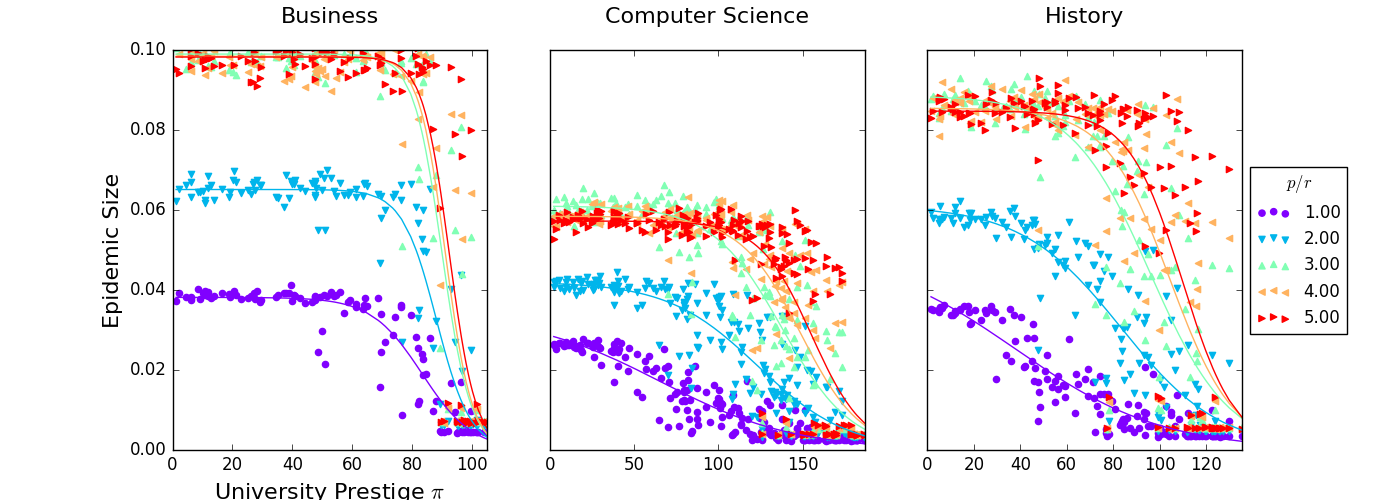
\includegraphics[width=\textwidth]{figures/size-results-of-ALL-SIS.png}
  \caption{Epidemic size versus prestige of the initially infected node under the SIS model, averaged over 500 trials.}
  \label{SIS-size}
\end{figure*}

\begin{figure*}
	\centering
  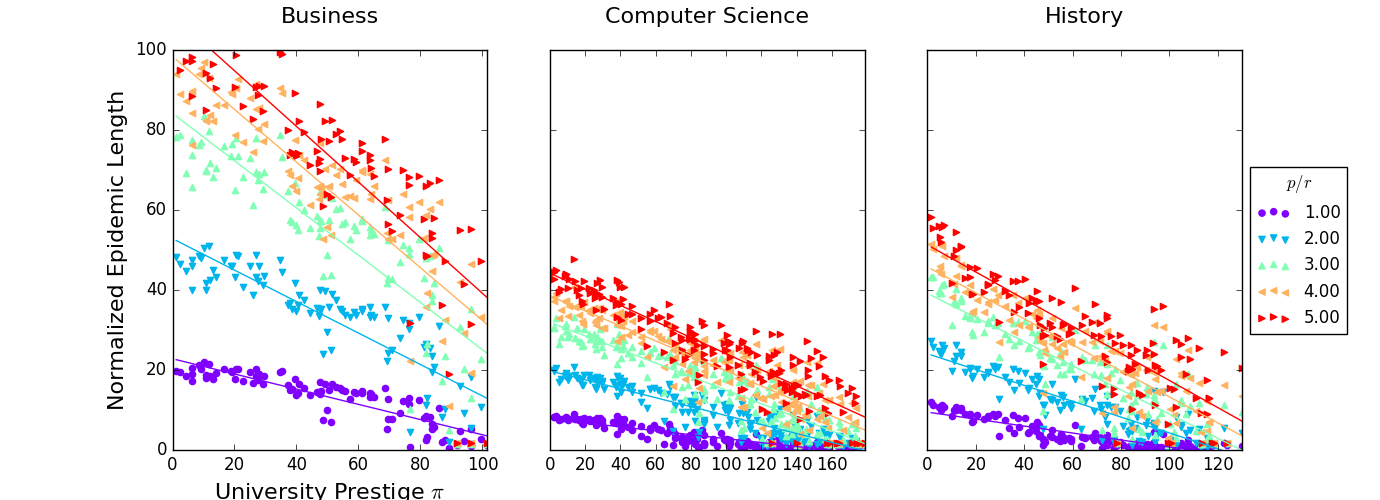
\includegraphics[width=\textwidth]{figures/length-results-of-ALL-SIS.png}
  \caption{Normalized epidemic length versus prestige of the initially infected node under the SIS model, averaged over 500 trials.}
   \label{SIS-length}
\end{figure*}

\subsection{\label{sec:level2}Random Jump}
In each of the disciplines, there are nodes that have no paths to large sections of the network. However, we expect that ideas starting at these fringe nodes should have at least a small chance to spread to those unreachable parts. In particular, in the lifetime of each epidemic, we allow each infected node $u$ to have exactly one chance (of probability $j$) of infecting a node selected uniformly at random from $u$'s set of unreachable nodes. (This approach is akin to the ``teleportation'' probability of a random walker within PageRank \cite{page:rank}.) Here we study how much of an effect this modification to our models has on epidemics. Please see figures~\ref{SI-random-size},~\ref{SIR-random-size}, and~\ref{SIS-random-size} for the results of this adjustment for SI, SIR, and SIS, respectively. The main insight we gain from these results are that increasing the jump probability $j$ has the largest effect on epidemic size for the lowest prestige institutions (those in the periphery). This is because those institutions now have a small chance of spreading their idea to a higher prestige, better connected, and therefore more influential institution. On the other hand, increasing jump probability does not affect the epidemic size for the highest prestige institutions because they are already in a central location at the core of the networks.

\begin{figure*}
	\centering
  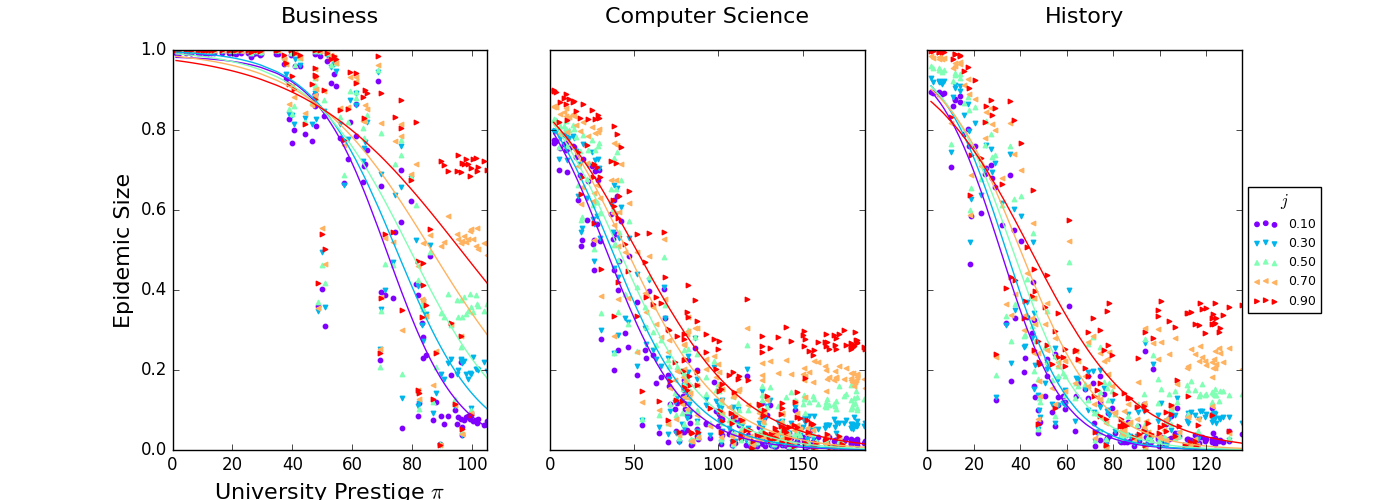
\includegraphics[width=\textwidth]{figures/size-results-of-ALL-SI-random-hops.png}
  \caption{Epidemic size versus prestige of the initially infected node under the SI model, allowing for a single jump to a disconnected node. Infection probability is held constant at $p = 0.1$. Each data point represents an average over 500 trials. Colors correspond to different jump probabilities.}
   \label{SI-random-size}
\end{figure*}

\begin{figure*}
	\centering
  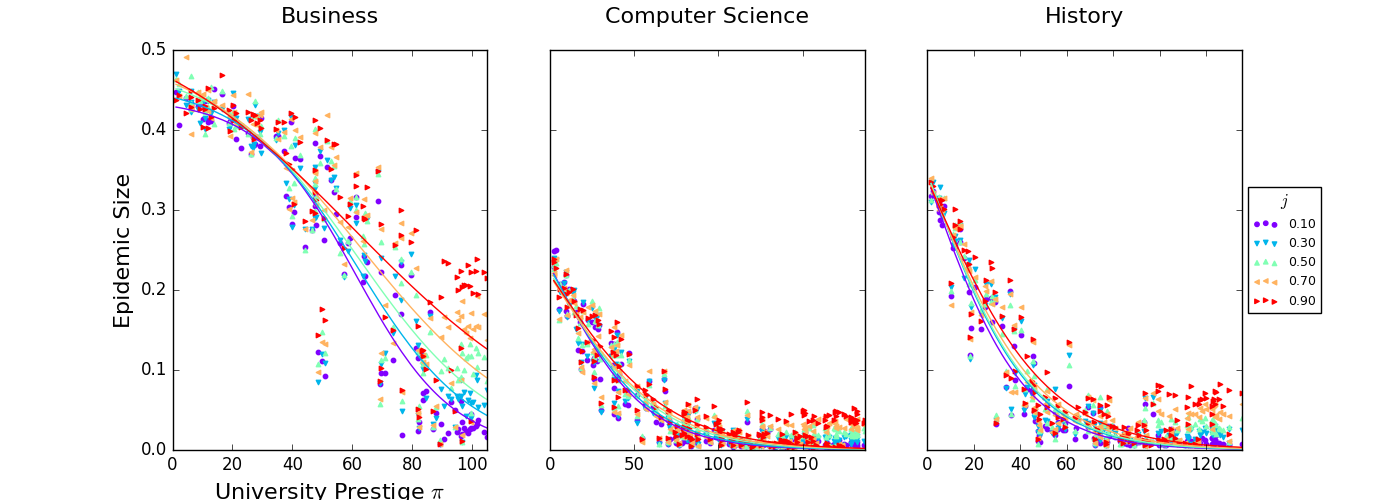
\includegraphics[width=\textwidth]{figures/size-results-of-ALL-SIR-random-hops.png}
  \caption{Epidemic size versus prestige of the initially infected node under the SIR model, allowing for a single jump to a disconnected node. Infection and recovery probabilities are held constant at $p = 0.1$ and $r = 0.2$. Each data point represents and average over 250 trials.}
   \label{SIR-random-size}
\end{figure*}

\begin{figure*}
	\centering
  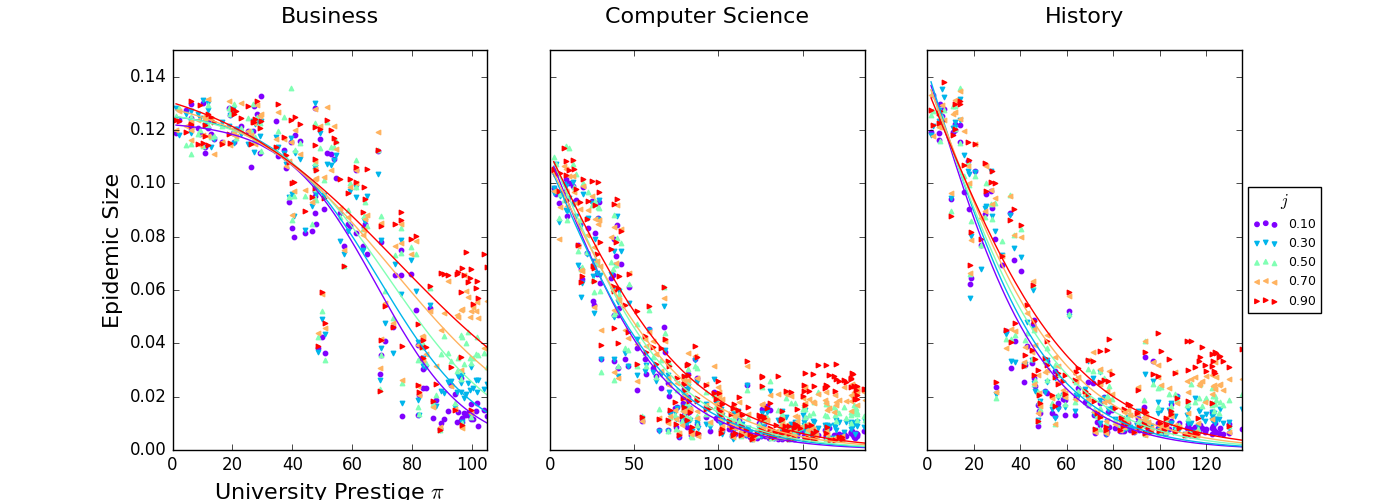
\includegraphics[width=\textwidth]{figures/size-results-of-ALL-SIS-random-hops.png}
  \caption{Epidemic size versus prestige of the initially infected node under the SIS model, allowing for a single jump to a disconnected node. Infection and recovery probabilities are held constant at $p = 0.1$ and $r = 0.2$. Each data point represents an average over 250 trials.}
   \label{SIS-random-size}
\end{figure*}

\subsection{\label{sec:infection}Relationship Between Prestige and Fitness of Idea}

In Fig.~\ref{SI-infection-size}, we have shown how epidemic size varies for increasing infection probability under the SI model. Each line corresponds to epidemic size averages over the universities in a particular prestige percentile. For example, the purple line includes the top 10\% of universities by prestige ranking. Fig.~\ref{SI-infection-size} suggests that research ideas stemming from the lowest prestige universities, even if they are of the highest quality, will never reach the whole network.

The relationship between epidemic size and infection probability (or fitness of a research idea) does not appear linear. Initial increases in infection probability have a larger impact on epidemic size than the same increase would have at larger infection probabilities. This trend might make some sense in the real world: research above some reader's quality threshold might still be deemed quality research.

The same figure allows us to assess how much fitter ideas starting in lower prestige universities need to be in order to reach as many universities as ideas starting from the higher prestige universities. For example, in the history plot, we have drawn a horizontal gray line for $\text{size} = 0.8$ (representing ideas spreading to $80$\% of the network). Based on this line, an idea starting from a top 10\% university only needs a fitness of about $0.10$ to reach $80$\% of the network, whereas an idea starting from a mid-rank institution needs a fitness of about $0.42$ to reach $80$\% of the network, i.e. it needs to be more than four times as fit. Furthermore, an idea starting from a bottom 20\% university can not even reach $80$\% of the network.  

By more closely inspecting the data, we can also generally conclude that ideas starting from universities in the top 10\% need only be as fit as $0.40$, $0.90$, and $0.70$ across business, computer science and history departments, respectively, to reach the whole network (i.e., cause an epidemic size of $1.00$). Yet universities in the 50th percentile need their ideas to be as fit as $0.70$, $1.00$ and $1.00$ across the same departments, respectively. This result suggests that ideas originating in the periphery need to be $1.75$, $1.11$ and $1.43$ times fitter, for each discipline respectively, than those originating in the core, in order to have success in spreading to all institutions.

\begin{figure*}
	\centering
  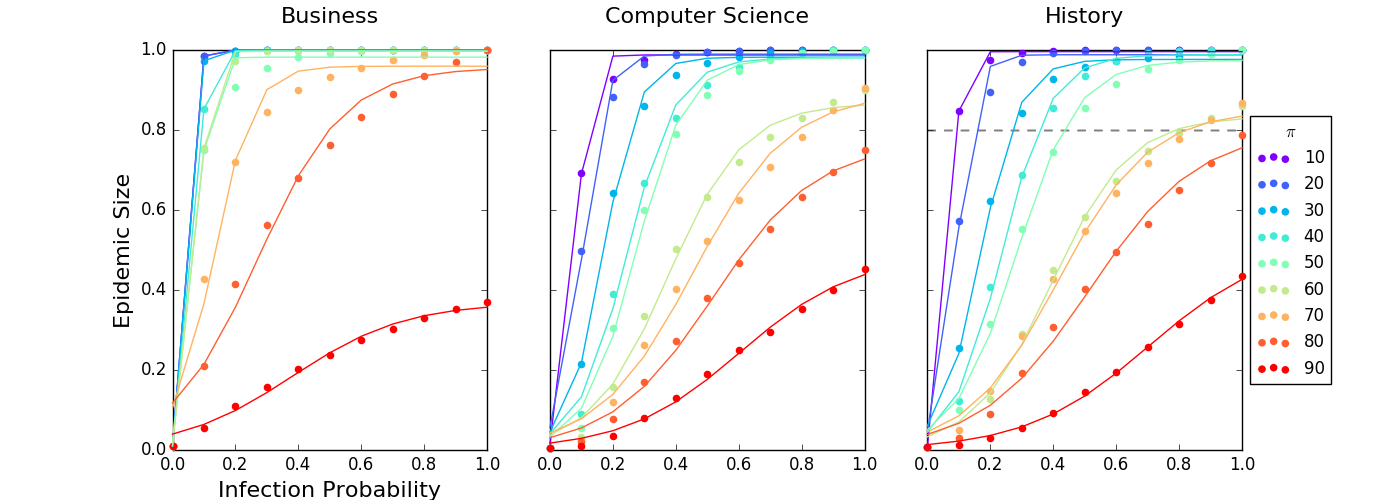
\includegraphics[width=\textwidth]{figures/infectious-size-results-of-ALL-SI.png}
  \caption{Epidemic size versus infection probability for each university by prestige percentile.}
  \label{SI-infection-size}
\end{figure*}

\section{\label{sec:level1}Conclusion}

In this paper, we investigated how university prestige affects epidemic size and length. Across all three epidemic models, and all three departments, infections starting from higher prestige institutions resulted in larger epidemic sizes and longer epidemic lengths: they had more impact. We further saw that ideas starting in the periphery (lower prestige institutions) need to be much more fit to have similar success as less fit ideas originating in the core. This reflects the fact that idea spreading in faculty hiring networks is not meritocratic.

While these results are intuitive and expected from core-periphery networks, we would ultimately like to see if these models agree with real data representing ideas spreading among universities. Some ideas for additional data that might allow us to explore this direction are citation networks, collaboration networks, etc. Future work in this direction could involve collecting our own data by scraping conference attendance information, and studying their citation networks, where conferences determine paper quality (idea fitness). We could also investigate whether schools of similar prestige frequent the same conferences. By doing so, we could establish whether conference attendance networks exhibit a similar core-periphery structure to our faculty hiring networks. Part of this work would also likely require recasting our models so that the infection and recovery probabilities are described in terms of time.

If we took our research in this direction, it is plausible that we would also have to consider more epidemic models (in case the models we considered do not wholly or accurately reflect idea proliferation in faculty hiring networks). In any case, studying the behavior of different epidemic models on networks (a survey of which was done by Pastor-Satorras et al.~\cite{epidemicsurvey}) on these faculty hiring networks (as well as perhaps other core-periphery networks) would be an interesting exercise in itself. There is also a lot more work we can do with the so-called random jump models. We can explore a larger portion of its parameter space (for example, jump probability, number of random jumps attempted, etc.). Also, instead of this model, we initially considered what we call a \emph{weak-edged} epidemic model where, in addition to the original network structure, we add edges between every pair of nodes in the network with very small weight (relating to the small jump probabilities in our random jump model). We came up with the random jump model as an alternative to the weak-edge model because the latter was cost-prohibitive. In the future, we would like to consider the weak-edge model as well, and doing so would involve optimizing our code (and possibly writing it in a different language like C).

In the literature, there are other network properties that could help identify who the most influential nodes are. A typical strategy is to use $k$-cores to examine core-periphery structure, the usual strategy of which is described and extended by Rombach et al., for example~\cite{rombach:coreperiphery}. More recent results by Malliaros et al. show that certain properties of the $k$-truss decomposition (a triangle-based extension of the core decomposition of graphs) of networks greatly help in locating influential nodes in real-world networks~\cite{malliaros:influentialnodes}. It would be interesting to see if this agrees with our results where prestige locates influential nodes under the epidemic models we considered.

\begin{comment}
\appendix
\section{Python code for our epidemic models}
\lstinputlisting[style=custompython, columns=1]{epidemic.py}

\begin{comment}
\section{Lines of Best Fit}
\begin{table*}[]
\centering
\caption{Parameters for the lines of best for Fig. \ref{SI-size}}
\label{my-label}
\begin{tabular}{c|c|ccc}
\textbf{department}               & \bm{$p$} & \bm{$s_\text{max}$}     & $\bm{|k|}$     & \bm{$\pi_\textbf{half}$}     \\ \hline
\multirow{5}{*}{business}         & 0.1        & 0.96591056     & 0.09160447     & 71.09284471    \\
                                  & 0.3        & 0.98645531     & 0.20981606     & 85.75541579    \\
                                  & 0.5        & 0.99767174     & 0.2457385      & 88.78644802    \\
                                  & 0.7        & 1.             & 0.25398815     & 90.70301287    \\
                                  & 0.9        & 1.             & 0.25859073     & 92.13037394    \\ \hline
\multirow{5}{*}{computer science} & 0.1        & 0.93844376     & 0.04607179     & 35.59533871    \\
                                  & 0.3        & 1.00000000e+00 & 4.01927105e-02 & 1.05579830e+02 \\
                                  & 0.5        & 9.92998792e-01 & 5.33085380e-02 & 1.35013790e+02 \\
                                  & 0.7        & 9.99654632e-01 & 6.29370790e-02 & 1.47758629e+02 \\
                                  & 0.9        & 9.97249266e-01 & 7.82455238e-02 & 1.56246668e+02 \\ \hline
\multirow{5}{*}{history}          & 0.1        & 1.             & 0.07503051     & 30.18516077    \\
                                  & 0.3        & 1.00000000e+00 & 5.56736795e-02 & 7.21796471e+01 \\
                                  & 0.5        & 1.00000000e+00 & 6.49174038e-02 & 9.37253745e+01 \\
                                  & 0.7        & 9.88758167e-01 & 8.34062453e-02 & 1.04352274e+02 \\
                                  & 0.9        & 9.83126563e-01 & 1.08144119e-01 & 1.10652621e+02 \\ \hline
\end{tabular}
\end{table*}

\begin{table*}[]
\centering
\caption{Parameters for the lines of best for Fig. \ref{SIR-size}}
\label{my-label}
\begin{tabular}{c|c|ccc}
\textbf{department}               & \bm{$p/r$} & \bm{$s_\text{max}$}     & $\bm{|k|}$     & \bm{$\pi_\textbf{half}$}     \\ \hline
\multirow{5}{*}{business}         & 1.0          & 0.18657936     & 0.12361925     & 80.28253832    \\
                                  & 2.0          & 0.37609244     & 0.1910131      & 86.56605687    \\
                                  & 3.0          & 0.53722915     & 0.20834285     & 88.10355712    \\
                                  & 4.0          & 0.54069659     & 0.22329182     & 89.7355563     \\
                                  & 5.0          & 0.54263412     & 0.23402705     & 91.02527139    \\ \hline
\multirow{5}{*}{computer science} & 1.0          & 1.71922046e-01 & 2.97388287e-02 & 4.97260575e+01 \\
                                  & 2.0          & 3.12855443e-01 & 3.67736205e-02 & 1.09827590e+02 \\
                                  & 3.0          & 4.60633916e-01 & 4.67259648e-02 & 1.30134386e+02 \\
                                  & 4.0          & 4.78268539e-01 & 5.44821197e-02 & 1.42994894e+02 \\
                                  & 5.0          & 4.88168936e-01 & 6.44839148e-02 & 1.51051409e+02 \\ \hline
\multirow{5}{*}{history}          & 1.0          & 0.22219957     & 0.04103311     & 33.38481069    \\
                                  & 2.0          & 3.61067381e-01 & 4.55969766e-02 & 7.42770443e+01 \\
                                  & 3.0          & 5.02079727e-01 & 5.64702449e-02 & 8.96833158e+01 \\
                                  & 4.0          & 5.05264310e-01 & 6.72635546e-02 & 1.00179212e+02 \\
                                  & 5.0          & 5.02214348e-01 & 8.87264279e-02 & 1.07198948e+02 \\ \hline
\end{tabular}
\end{table*}

\begin{table*}[]
\centering
\caption{Parameters of for the lines of best fit for Fig. \ref{SIS-size}}
\label{my-label}
\begin{tabular}{c|c|ccc}
\textbf{department}               & \bm{$p/r$} & \bm{$s_\text{max}$}     & $\bm{|k|}$     & \bm{$\pi_\textbf{half}$}     \\ \hline
\multirow{5}{*}{business}         & 1.0          & 3.81519673e-02 & 1.18378693e-01 & 8.32270021e+01 \\
                                  & 2.0          & 6.51226855e-02 & 1.75962495e-01 & 8.80255119e+01 \\
                                  & 3.0          & 0.09897937     & 0.21061661     & 89.84536868    \\
                                  & 4.0          & 0.0984244      & 0.2256236      & 90.99530129    \\
                                  & 5.0          & 0.09824274     & 0.22504195     & 92.30123438    \\ \hline
\multirow{5}{*}{computer science} & 1.0          & 3.41033659e-02 & 2.50738777e-02 & 6.58760327e+01 \\
                                  & 2.0          & 4.20447186e-02 & 3.74828270e-02 & 1.23366607e+02 \\
                                  & 3.0          & 6.10054480e-02 & 4.83853147e-02 & 1.37814625e+02 \\
                                  & 4.0          & 5.84336643e-02 & 5.58916707e-02 & 1.48788396e+02 \\
                                  & 5.0          & 5.72453854e-02 & 6.42899958e-02 & 1.55506313e+02 \\ \hline
\multirow{5}{*}{history}          & 1.0          & 5.01674867e-02 & 3.18530317e-02 & 3.83563237e+01 \\
                                  & 2.0          & 6.11320656e-02 & 4.66829473e-02 & 8.34520322e+01 \\
                                  & 3.0          & 8.85683841e-02 & 5.87596949e-02 & 9.59482548e+01 \\
                                  & 4.0          & 8.54498232e-02 & 7.21429163e-02 & 1.04461455e+02 \\
                                  & 5.0          & 8.47266757e-02 & 8.69345706e-02 & 1.09799566e+02 \\ \hline
\end{tabular}
\end{table*}

\begin{table*}[]
\centering
\caption{Parameters for the lines of best fit for Fig. \ref{SI-length}}
\label{my-label}
\begin{tabular}{c|c|cc}
\textbf{department}               & \bm{$p$} & \bm{$m$}  & \bm{$b$} \\ \hline
\multirow{5}{*}{business}         & 0.1        & -0.03125012 & 4.30771565 \\
                                  & 0.3        & -0.01533506 & 3.07003648 \\
                                  & 0.5        & -0.00853344 & 2.52455467 \\
                                  & 0.7        & -0.00621331 & 2.36117491 \\
                                  & 0.9        & -0.00522434 & 2.28280288 \\ \hline
\multirow{5}{*}{computer science} & 0.1        & -0.02553816 & 3.99908591 \\
                                  & 0.3        & -0.01553432 & 3.4043385  \\
                                  & 0.5        & -0.00931224 & 2.8170329  \\
                                  & 0.7        & -0.00610161 & 2.46044653 \\
                                  & 0.9        & -0.00405643 & 2.22605227 \\ \hline
\multirow{5}{*}{history}          & 0.1        & -0.03404618 & 3.81866688 \\
                                  & 0.3        & -0.02139187 & 3.300967   \\
                                  & 0.5        & -0.0134275  & 2.81142342 \\
                                  & 0.7        & -0.00884088 & 2.46918606 \\
                                  & 0.9        & -0.0060994  & 2.26040899 \\ \hline
\end{tabular}
\end{table*}

\begin{table*}[]
\centering
\caption{Parameters for the lines of best fit for Fig. \ref{SIR-length}}
\label{my-label}
\begin{tabular}{c|c|cc}
\textbf{department}               & \bm{$p/r$} & \bm{$m$}  & \bm{$b$} \\ \hline
\multirow{5}{*}{business}         & 1.0          & -0.01039302 & 2.0185306  \\
                                  & 2.0          & -0.00815439 & 2.10290138 \\
                                  & 3.0          & -0.00721221 & 2.15768384 \\
                                  & 4.0          & -0.00543295 & 2.03086031 \\
                                  & 5.0          & -0.00475224 & 1.97280466 \\ \hline
\multirow{5}{*}{computer science} & 1.0          & -0.00986126 & 2.04048956 \\
                                  & 2.0          & -0.0085257  & 2.2896116  \\
                                  & 3.0          & -0.007591   & 2.35554319 \\
                                  & 4.0          & -0.00520269 & 2.10078136 \\
                                  & 5.0          & -0.0036817  & 1.92599271 \\ \hline
\multirow{5}{*}{history}          & 1.0          & -0.01316831 & 1.97239641 \\
                                  & 2.0          & -0.01195739 & 2.26701795 \\
                                  & 3.0          & -0.01092811 & 2.35278644 \\
                                  & 4.0          & -0.00772274 & 2.11820239 \\
                                  & 5.0          & -0.00572671 & 1.96423557 \\ \hline
\end{tabular}
\end{table*}

\begin{table*}[]
\centering
\caption{Parameters for the lines of best fit for Fig. \ref{SIS-length}}
\label{my-label}
\begin{tabular}{c|c|cc}
\textbf{department}               & \bm{$p/r$} & \bm{$m$}  & \bm{$b$} \\ \hline
\multirow{5}{*}{business}         & 1.0          & -0.19001202 & 22.80498734  \\
                                  & 2.0          & -0.39341598 & 52.84230751  \\
                                  & 3.0          & -0.59090523 & 84.14501818  \\
                                  & 4.0          & -0.65979504 & 98.3509927   \\
                                  & 5.0          & -0.69559229 & 108.72260089 \\ \hline
\multirow{5}{*}{computer science} & 1.0          & -0.04926305 & 7.76497291   \\
                                  & 2.0          & -0.11187941 & 19.79276682  \\
                                  & 3.0          & -0.16968724 & 31.92269492  \\
                                  & 4.0          & -0.18762018 & 38.5190345   \\
                                  & 5.0          & -0.20118842 & 44.1980368   \\ \hline
\multirow{5}{*}{history}          & 1.0          & -0.08700149 & 9.46354689   \\
                                  & 2.0          & -0.19802986 & 24.07374589  \\
                                  & 3.0          & -0.3015026  & 39.14360718  \\
                                  & 4.0          & -0.32490024 & 45.78110042  \\
                                  & 5.0          & -0.33885474 & 51.2793859   \\ \hline
\end{tabular}
\end{table*}

\begin{table*}[]
\centering
\caption{Parameters for lines of best fit for Fig. \ref{SI-infection-size}}
\label{my-label}
\begin{tabular}{c|c|ccc}
\textbf{department}               & \bm{$\pi\textbf{ (percentile)}$}             & \bm{$s_\textbf{max}$}     & \bm{$k$}      & \multicolumn{1}{l}{\bm{$\pi_\textbf{half}$}} \\ \hline
\multirow{9}{*}{business}         & 10                      & 9.99818624e-01 & 8.90788277e+01 & 5.28668159e-02        \\
                                  & 20                      & 9.99828808e-01 & 8.89333015e+01 & 5.29534503e-02        \\
                                  & 30                      & 9.99817357e-01 & 8.30253453e+01 & 5.67204311e-02        \\
                                  & 40                      & 0.99866752     & 64.3890176     & 0.07259215            \\
                                  & 50                      & 0.98216266     & 52.46554384    & 0.07781178            \\
                                  & 60 & 0.9968616      & 56.0264262     & 0.07975508            \\
                                  & 70 & 0.95951299     & 16.07436548    & 0.1300846             \\
                                  & 80 & 0.95613664     & 7.23965066     & 0.27159736            \\
                                  & 90 & 0.36844533     & 5.55505975      & 0.38087751            \\ \hline
\multirow{9}{*}{computer science} & 10                      & 0.98763526     & 49.66853395    & 0.08304112            \\
                                  & 20                      & 0.98958845     & 27.21740565    & 0.10276491            \\
                                  & 30                      & 0.98201721     & 17.91609778    & 0.16993479            \\
                                  & 40                      & 0.98033725     & 12.8196032     & 0.24466168            \\
                                  & 50                      & 0.9804206      & 12.34154277    & 0.27255169            \\
                                  & 60 & 0.86701272     & 8.275734       & 0.37516933            \\
                                  & 70 & 0.89090447     & 6.57992448     & 0.45632556            \\
                                  & 80 & 0.76655679     & 6.09334345     & 0.51996798            \\
                                  & 90 & 0.48876615     & 5.47160704     & 0.60440341            \\ \hline
\multirow{9}{*}{history}          & 10                      & 0.99592456     & 66.07423453    & 0.07363681            \\
                                  & 20                      & 0.98810198     & 32.36682888    & 0.09211107            \\
                                  & 30                      & 0.97644993     & 16.0343579     & 0.16941897            \\
                                  & 40                      & 0.9884798      & 12.79924251    & 0.23716342            \\
                                  & 50                      & 0.97438401     & 10.31361185    & 0.28247904            \\
                                  & 60 & 0.83399479     & 8.07554255     & 0.39526119            \\
                                  & 70 & 0.84948519     & 6.91606226     & 0.41674393            \\
                                  & 80 & 0.80154317     & 5.77212675     & 0.51530652            \\
                                  & 90 & 0.51913938     & 5.14863162     & 0.70341988            \\ \hline
\end{tabular}
\end{table*}
\end{comment}

\bibliography{main}
\bibliographystyle{plain}

\end{document}
%
% ****** End of file apssamp.tex ******